\begin{tcolorbox}[breakable,colback=black!5!white,colframe=red!80!black,width=\textwidth]
\chapter{Theoretical motivation}
\end{tcolorbox}
\label{chap:theory}

The Standard Model (SM) of particles represents, so far, the best available description of the particles and their interactions. It is the summation of two gauge theories: the electroweak interaction, that pictures together the weak and electromagnetic interactions, and the strog interaction, or Quantum Chromodynamics (QCD). Particles, namely quarks and leptons, are described by spin 1/2 fermions, whilst interactions are embodied by spin 1 bosons. The simmetry group of the standard model is:
\begin{equation}
SU_{C}(3) \times SU_L (2) \times U_Y (1),
\end{equation}
\label{eq:theory_SMgroup}
where the first factor is related to strong interactions, whose mediators are eight gluons, whilst $SU_L (2) \times U_Y (1)$ is the electroweak simmetry group, whose mediators are photons and $Z$-$W^{\pm}$ bosons.

In renormalizable theories, with no anomalies, all gauge bosons are expected to be massless, in contrast with our experimental knowledge (cite W-Z discovery). This kind of dilemma can be solved by introducing a new scalar particle, the Higgs boson (cite Higgs article), that can give mass to weak bosons and fermions via the spontaneous symmetry breaking mechanism.

In the last decades, Standard Model has been accurately probed by many experimental facilities (LEP, Tevatron), demonstrating an impressive agreement between theoretical predictions and experimental results. The discovery of the Higgs boson at the CERN Large Hadron Collider, measured by both CMS and ATLAS collaborations~\cite{bib:Aad20121,bib:Chatrchyan201230,bib:Chatrchyan2013lba,Aad:2013xqa,Khachatryan:2014jba,Aad:2014aba,Aad:2015zhl}, represents not only an extraordinary confirmation of the model, but also the latest biggest achievement in particle physics as a whole.

\section{Beyond Standard Model theories}
Even though the Standard Model is the most complete picture of the universe of the particles, many questions are still left open by the model. From a phenomenological point of view, some experimental observations are not included in the theory:
\begin{itemize}
\item in SM, neutrinos are massless (whilst experimentally it has been confirmed to be non-zero, i.e. by the neutrino oscillation);
\item no candidate for the dark matter is foreseen (whilst it has been observed in cosmology);
\item no fields included in the SM can explain the cosmological inflation;
\item SM can not justify the matter-antimatter asymmetry.
\end{itemize}
From a purely theoretical perspective, some issues are still relevant in the formulation of the model:
\begin{itemize}
\item {\itshape Flavour problem.}\\ The Standard Model has 18 free parameters: 9 fermionic masses; 3 angular parameters in Cabibbo-Kobayashi-Maskawa matrix, plus 1 phase parameter; electromagnetic coupling $\alpha$; strong coupling $\alpha_{strong}$;  weak coupling $\alpha_{weak}$; $Z$ mass; the mass of the Higgs boson. Such a huge number of degrees of freedom is considered as weakly predictive.
\item {\itshape Unification.}\\ There is not a ``complete'' unification of strong, weak and electromagnetic interactions, since each one has its own coupling constant, behaving differently at different energy scales; not to mention the fact that gravitational interaction, completely excluded from the SM.
\item {\itshape Hierarchy problem.}\\ From Quantum Field Theory, it is known that perturbative corrections to the mass of the scalar bosons included in the theory tend to make it increase towards the energy scale at which the considered theory is valid [cite n. 4 of master thesis]. If the Standard Model is seen as a low-mass approximation of a more general theory valid uo to the Planck mass scale (i.e., $\approx 10^{19}$ GeV), a fine-tuning cancellation of the order of $1$ over $10^{34}$ is needed in order to protect the Higgs mass at the electroweak scale ($\approx 100$ GeV). Such an astonishing correction is perceived as very unnatural.
%\item {\itshape Problema della scala delle masse.}\\ Perch\'e nel Modello Standard le masse delle particelle fermioniche vanno dall'ordine dell'eV per i neutrini (limite forse molto sovrastimato, come emerge dalle differenze di massa nelle oscillazioni) alla centinaia di GeV del quark top?
\end{itemize}

Numerous Beyond Standard Model theories (BSM) have been proposed in order to overcome the limits of the Standard Model.

Grand Unified Theories (GUT) aim at extending the symmetry group of the SM (eq.~\ref{eq:theory_SMgroup}) into largest candidates, such as $S0(10)$, $SU(5)$ and $E(6)$. At GUT scale, approximately at $10^{16}$ GeV, non-gravitational interactions are expected to be ruled by only one coupling constant, $\alpha_{GUT}$. %Pur godendo di alcuni punti di forza, quali la possibilit\`a di dare massa ai neutrini ammettendo l'esistenza del neutrino right alla scala GUT, queste teorie prevedono in alcuni casi fenomeni non ancora osservati (decadimento del protone, esistenza dei monopoli magnetici) e sono valide ad energie non riproducibili sperimentalmente. Qualche speranza di trovare nuova fisica a scale inferiori potrebbe nascere dal connubio tra GUT e modelli supersimmetrici.

Super Symmetryc (SUSY) models state that every fermion (boson) of the Standard Model has a bosonic (fermionic) superpartner, with exactly the same quantum numbers, except the spin. If SUSY is not broken, each couple of partners and superpartners should have the same masses, hypotesis easily excluded by the non-observation of the s-electron. Super Symmetry represents a very elegant solution of the hierarchy problem of the Higgs boson mass, since the perturbative corrections brought by new SUSY particles exactly cancel out the divergences caused by SM particles corrections. A particular sub-class of SUSY models, Minimal Super Symmetric Standard Models, is characterized by the introduction of a new symmetry, the R-parity, that guarantees the proton stability and also the stability of the lightest SUSY particle, a possible good candidate for dark matter.

Two other possible theoretical pictures are extensively described in sec.~\ref{sec:theory_HVT}-\ref{sec:theory_WED}.

\newpage

\section{Heavy Vector Triplet}
\label{sec:theory_HVT}

The heavy vector triplet model~\cite{Pappadopulo2014} provides a general framework aimed at studying new physics beyond the standard model, that can manifest into the appearance of new resonances.\\
The adopted approach is that of the simplified model, in which an effective Lagrangian is introduced, in order to describe the properties and interactions of new particles (in this case, a triplet of spin-1 bosons) by using a limited set of parameters, that can be easily linked to the physical observables at the LHC experiments. These parameters can describe many physical motivated theories (such as sequential extensions of the SM~\cite{Barger:1980ix,Grojean:2011vu} or Composite Higgs~\cite{Contino2011,Bellazzini:2014yua}). \\
Since a simplified model is not a complete theory, its validity is restricted to the on-shell quantities related to the production and decay mechanisms of new resonances, that is the case of most of the LHC BSM searches are performed. Given these conditions, experimental results in the resonant region are sensitive to a limited number of the phenomenological Lagrangian parameters (or to a combination of those), whilst the remaining parameters tend to influence the tail of the distributions.\\
Limits on production cross-section times branching ratio ($\sigma  \mathcal{B}$), as a function of the invariant mass spectrum of the probed resonance, can be extracted from experimental data. Given that $\sigma  \mathcal{B}$ are functions of the simplified model parameters and of the parton luminosities, it is then possible to interpret the observed limits in the parameter space.

\subsection{Simplified Lagrangian}
\label{sec:HVT_lagr}

The heavy vector triplet framework assumes the existence of an additional vector triplet, $V_{\mu}^a$, $a=1,2,3$, in which two spin-1 particles are charged and one is neutral:

\begin{equation}
V_{\mu}^{\pm} = \frac{V_{\mu}^1 \mp i V_{\mu}^2}{\sqrt{2}}; \mbox{ } V_{\mu}^0 = V_{\mu}^3.
\label{eq:V_triplet}
\end{equation}
\\
The triplet interactions are described by a simplified Lagrangian, that is invariant under SM gauge and CP symmetry, and accidentally invariant under the custodial symmetry $SU(2)_L \times SU(2)_R$:
\begin{equation}
\begin{split}
\mathcal{L_V} ={} & -\frac{1}{4} \left(D_{\mu}V_{\nu}^a - D_{\nu}V_{\mu}^a \right) \left( D^{\mu}V^{\nu \mbox{ } a} - D^{\nu}V^{\mu \mbox{ } a} \right) + \frac{m_V^2}{2}V_{\mu}^aV^{\mu \mbox{ } a} \\
 & +i g_V c_H V_{\mu}^a \left( H^{\dagger} \tau^a D^{\mu}H - D^{\mu}H^{\dagger} \tau^a H \right) + \frac{g^2}{g_V}c_F V_{\mu}^a \sum_{f} \bar{f}_L \gamma^{\mu} \tau^a f_L \\
 & + \frac{g_V}{2} c_{VVV} \epsilon_{abc} V_{\mu}^a V_{\nu}^b \left( D^{\mu}V^{\nu \mbox{ } c} - D^{\nu}V^{\mu \mbox{ } c}\right) + g_V^2 c_{VVHH} V_{\mu}^a V^{\mu \mbox{ } a} H^{\dagger} H - \frac{g}{2} c_{VVW} \epsilon_{abc} W^{\mu \nu \mbox{ } a} V_{\mu}^b V_{\nu}^c.
\end{split}
\label{eq:Lagrangian}
\end{equation}
\\
In the first line of the formula~\ref{eq:Lagrangian}, $V$ mass and kinematic terms are included, described with the covariant derivative $D_{\mu} V_{\nu}^a = \partial_{\mu} V_{\nu}^a + g \epsilon^{abc} W_{\mu}^b V_{\nu}^c$, where $W_{\mu}^a$ are the fields of the weak interaction and $g$ is the weak gauge coupling. $V_{\mu}^a$ are not mass eigenstates, since they mix with the electroweak fields after the spontaneous symmetry breaking, therefore $m_V$ isn't the physical mass of the $V$ bosons.\\
The second line describes the interaction of the triplet with the Higgs field and the SM left-handed fermions; $c_H$ describes the vertices with the physical Higgs and the three unphysical Goldstone bosons that, for the Goldstone equivalence theorem, are connected to the longitudinal polarization of W and Z bosons at high-energy; hence, $c_H$ is related to the bosonic decays of the resonances. $c_F$ is the analogous parameter describing the $V$ interaction with fermions, that can be generalized as a flavour dependent coefficent, once defined $J_F^{\mu \mbox{ } a} = \sum_{f} \bar{f}_L \gamma^{\mu} \tau^a f_L$: $c_F V_{\mu}^a  J_F^{\mu \mbox{ } a} = c_{\ell} V_{\mu}^a  J_{\ell}^{\mu \mbox{ } a} + c_{q} V_{\mu}^a  J_{q}^{\mu \mbox{ } a} + c_{3} V_{\mu}^a  J_{3}^{\mu \mbox{ } a}$.\\
The last part of the equation includes terms that are relevant only in strongly coupled scenarios (see sec.~\ref{sec:HVT_decay_bosons}) through the $V$-$W$ mixing, but it does not include vertices of $V$ with light SM fields, hence it can be neglected while describing the majority of the LHC phenomenology, under the assumptions previously stated. Additional dimension four quadrilinear $V$ interactions are non relevant for the processes discussed, otherwise their effects would be appreciated in electroweak precision tests and precise Higgs coupling measurements~\cite{Giudice:2007fh}.\\

The parameters in the Lagrangian can be interpreted as follows: $g_V$ describes the strenght of the interaction, that is weighted by $c$ parameters. $g_V$ ranges from $g_V \sim 1$ when the coupling is weak (sec. \ref{sec:theory_HVT_A}), to $g_V \sim 4 \pi$ when the coupling is strong (sec. \ref{sec:theory_HVT_B}). $c$ parameters are expected to be $c \sim 1$, except to $c_H$, that can be smaller for weak couplings. The combinations describing the vertices, $g_V c_H$ and $g^2/g_v c_F$, can be considered as the fundamental parameters, used to interpret the experimental results.

\subsection{Mass eigenstates, mixing parameters and decay widths}
\label{sec:HVT_pheno}

The newly introduced $SU(2)_L$ triplet is expected to mix with the weak SM fields. The $U(1)_{em}$ symmetry is left unbroken by the new interaction, hence the massless combination of the electroweak fields, namely the photon, is the same as the SM:
\begin{equation}
A_{\mu} = B_{\mu} \cos{\theta_W} + W_{\mu}^3 \sin{\theta_W},
\label{eq:A_mu}
\end{equation} 
with the usual definitions of the electroweak parameters:
\begin{equation}
\begin{split}
 & \tan{\theta_W}=\frac{g'}{g} \\
 & e = \frac{g g'}{\sqrt{g^2 + {g'}^2}} \\
 & g = e/\sin{\theta_w}; g' = e/\cos{\theta_w}.
\end{split}
\label{eq:ewk_param}
\end{equation}

The $Z$ boson, on the other hand, mixes with the neutral component of the triplet, $V^0$, with a rotation parametrized with the angle $\theta_N$:
\begin{equation}
\begin{pmatrix}
\cos{\theta_N} & \sin{\theta_N} \\
-\sin{\theta_N} & \cos{\theta_N}d \\
\end{pmatrix}
\begin{pmatrix}
Z  \\
V^0  \\
\end{pmatrix}
.
\label{eq:mixing}
\end{equation}
The mass matrix of the rotated system is given by:
\begin{equation}
\mathbb{M}_N^2 =
\begin{pmatrix}
\hat{m}_Z^2 & c_H \zeta \hat{m}_Z \hat{m}_V \\
c_H \zeta \hat{m}_Z \hat{m}_V & \hat{m}_V^2 \\
\end{pmatrix}
,
\label{eq:mass_matrix_Z}
\end{equation}
where the parameters are defined as:
\begin{equation}
\left\{
\begin{array}{l}
\hat{m}_Z = \frac{e}{2 \sin{\theta_W} \cos{\theta_W}}\hat{v} \\
\hat{m}_V^2 = m_V^2 + g_V^2 c_{VVHH} {\hat{v}}^2\\
\zeta = \frac{g_V \hat{v}}{2 \hat{m}_V}\\
\frac{\hat{v}^2}{2} = \langle H^{\dagger} H \rangle
\end{array},
\right.
\label{eq:mass_matrix_param_Z}
\end{equation}
and $\hat{v}$, the vacuum expectation value of the Higgs field, can be different from the SM $v = 246$ GeV. The physical masses of $Z$ and $V^0$, $m_Z$ and $M_0$, and $\theta_N$ come from the matrix relations:
\begin{equation}
\begin{split}
 & \mbox{Tr}\left( \mathbb{M}_N^2 \right) = \hat{m}_Z^2 + \hat{m}_V^2 = m_Z^2 + M_0^2\\
 & \left\| \mathbb{M}_N^2 \right\| = \hat{m}_Z^2 + \hat{m}_V^2 \left( 1 - c_H^2 {\zeta}^2\right) = m_Z^2 M_0^2 \\
 & \tan{2 \theta_N} = \frac{2 c_H \zeta \hat{m}_Z \hat{m}_V}{\hat{m}_V^2 - \hat{m}_Z^2}.
\end{split}
\label{eq:mass_eig_Z}
\end{equation}
%\\
%Given that $\hat{m}_V > \hat{m}_Z$, the tangent in eq.\ref{eq:mass_eig} is bijective.

The $W^{\pm}$ bosons mix with the charged components of the triplet, $V^{\pm}$, leading to a mass matrix analogous to eq.~\ref{eq:mass_matrix_Z}:
\begin{equation}
\mathbb{M}_C^2 =
\begin{pmatrix}
\hat{m}_W^2 & c_H \zeta \hat{m}_W \hat{m}_V \\
c_H \zeta \hat{m}_W \hat{m}_V & \hat{m}_V^2 \\
\end{pmatrix}
,
\label{eq:mass_matrix_Z}
\end{equation}
where $\hat{m}_W$ is defined as:
\begin{equation}
\left\{
\begin{array}{l}
\hat{m}_W = \frac{e}{2 \sin{\theta_W}} \hat{v} = \hat{m}_Z \cos{\theta_W} \\
\end{array};
\right.
\label{eq:mass_matrix_param_W}
\end{equation}
the physical masses of $W$ and $V^{\pm}$, $m_W$ and $M_{\pm}$, and the angle $\theta_C$ parametrizing the rotation of the charged sector are described by:
\begin{equation}
\begin{split}
 & \mbox{Tr}\left( \mathbb{M}_C^2 \right) = \hat{m}_W^2 + \hat{m}_V^2 = m_W^2 + M_{\pm}^2\\
 & \left\| \mathbb{M}_C^2 \right\| = \hat{m}_W^2 + \hat{m}_V^2 \left( 1 - c_H^2 {\zeta}^2\right) = m_W^2 M_{\pm}^2 \\
 & \tan{2 \theta_C} = \frac{2 c_H \zeta \hat{m}_W \hat{m}_V}{\hat{m}_V^2 - \hat{m}_W^2}.
\end{split}
\label{eq:mass_eig_W}
\end{equation}

The custodial symmetry of eq.~\ref{eq:Lagrangian} guarantees that:
\begin{equation}
\mathbb{M}_C^2 =
\begin{pmatrix}
\cos{{\theta}_W} & 0 \\
0 & 1 \\
\end{pmatrix}
\mathbb{M}_N^2
\begin{pmatrix}
\cos{{\theta}_W} & 0 \\
0 & 1 \\
\end{pmatrix}
.
\label{eq:custodial_matrix}
\end{equation}
\\
By taking the determinant of this matrices, a custodial relation among the masses can be extracted:
\begin{equation}
m_W^2 M_{\pm}^2 = \cos{{\theta}_W} m_Z^2 M_0^2,
\label{eq:custodial_relation}
\end{equation}
that has some very important consequences.\\
Given that this model aims at searching new particles in the TeV scale and that the scale of the electroweak interactions must lay at $\sim 100$ GeV,  a hierarchy of the physical masses seems very natural:
\begin{equation}
\frac{\hat{m}_{(W,Z)}}{\hat{m}_V} \sim \frac{{m}_{(W,Z)}}{M_{(\pm, 0)}} \ll 1
;
\label{eq:mass_hierarchy}
\end{equation}
$\zeta$ parameter can be $\zeta \ll 1$ (weakly coupled scenario) or $\zeta \sim 1$ (strongly coupled scenario). When eq.~\ref{eq:mass_hierarchy} applies, the second lines in eq.~\ref{eq:mass_eig_Z} and eq.~\ref{eq:mass_eig_W} can be approximated as follows:
\begin{equation}
\begin{split}
& m_Z^2 = \hat{m}_Z^2 \left( 1 - c_H^2 {\zeta}^2\right) \left( 1 + \mathcal{O}(\hat{m}_Z^2/\hat{m}_V^2) \right) \\
& m_W^2 = \hat{m}_W^2 \left( 1 - c_H^2 {\zeta}^2\right) \left( 1 + \mathcal{O}(\hat{m}_W^2/\hat{m}_V^2) \right) \\
\end{split}
.
\label{eq:mass_simpl}
\end{equation}
\\
From eq.~\ref{eq:mass_matrix_param_W}, the ratio of the physical masses of the charged and neutral electroweak bosons can be approximated as:
\begin{equation}
\frac{m_W^2}{m_Z^2} \approx {\cos{{\theta}_W}}^2,
\label{eq:mass_ewk_ratio}
\end{equation}
that satisfies the SM tree-level relation $\rho = 1$ if ${\cos{{\theta}_W}}^2 \approx 1. - 0.23$. Adding this approximation into eq.~\ref{eq:custodial_relation}, the $V$ bosons are expected to have the same masses, hence the same production rates:
\begin{equation}
M_{\pm}^2 = M_0^2 \left(1 + \mathcal{O}(\%) \right).
\label{eq:HVT_degeneracy}
\end{equation}
The degenerate mass of the triplet will be called $M_V \approx M_{\pm} \approx M_0$; given~\ref{eq:mass_hierarchy}, $M_V = \hat{m}_V$.
\\
Another consequence of the mass hierarchy~(\ref{eq:mass_hierarchy}) is that the mixing angles $\theta_{(N,C)}$ between the electroweak fields and the triplet are small:
\begin{equation}
{\theta}_{(N,C)} \approx c_H \zeta \frac{\hat{m}_{(W,Z)}}{ \hat{m}_V } \ll 1,
\label{eq:HVT_small_angles}
\end{equation}
hence the couplings among SM particles are very close to the couplings predicted by the SM.

%\vspace*{1\baselineskip}
\subsubsection{Decay widths into fermions}
\label{sec:HVT_decay_fermions}

The couplings among the triplet and SM fermions are expressed as a function of the rotational parameters $\theta_{(C,N)}$ and SM couplings (omitting the CKM matrix elements for quarks):
\begin{equation}
\begin{split}
&
\left\{
\begin{array}{l}
g_L^N = \frac{g^2}{g_V} \frac{c_F}{2} \cos{{\theta}_N} + \left( g_L^Z \right)_{SM} \sin{{\theta}_N} \approx \frac{g^2}{g_V} \frac{c_F}{2} \\
g_R^N = \left( g_R^Z \right)_{SM} \sin{{\theta}_N} \approx 0\\
\end{array}
\right.
,\\
&
\left\{
\begin{array}{l}
g_L^C = \frac{g^2}{g_V} \frac{c_F}{2} \cos{{\theta}_C} + \left( g_L^W \right)_{SM} \sin{{\theta}_N} \approx \frac{g^2}{g_V} \frac{c_F}{2} \\
g_R^C = 0\\
\end{array}
\right.
,\\
\end{split}
\label{eq:HVT_couplings}
\end{equation}
where $g_L^W = g/2$. The $V$ bosons interact with SM left fermions, and the strenght of the couplings with fermions is determined by $g^2/g_V c_F$, as stated in sec.~\ref{sec:HVT_lagr}. The decay width into fermions is then given by:
\begin{equation}
\Gamma_{V^{\pm} \rightarrow f \bar{f'}} \approx 2 \Gamma_{V^{0} \rightarrow f \bar{f}} \approx N_c {\left( \frac{g^2 c_F}{g_V}\right)}^2 \frac{M_V}{48 \pi},
\label{eq:HVT_width_fermions}
\end{equation}
where $N_c$ is the number of colours (3 for quarks, 1 for leptons).

\subsubsection{Decay widths into bosons}
\label{sec:HVT_decay_bosons}
As a starting point, a proper choice of the gauge makes easier the derivation of approximate decay widths. While the unitary gauge is very convenient in discussing the electroweak symmetry breaking mechanism, since it provides a basis in which the Goldstone components of the scalar fields of the theory are set to zero, it does not properly describe the logitudinally polarized bosons in high-enery regimes, since it introduces a dependence of the type $E/m$ in the logitudinal polarization vector, not corresponding to the experimental results. This pathological behaviour can be overcome profiting of the equivalence theorem: while calculating the scattering amplitude of an high-energy process, the longitudinally polarized vectors are equivalent to their corresponding Goldstone scalars. The scattering amplitude can therefore be calculated with Goldstone diagrams.\\
In the so-called equivalent gauge~\cite{Wulzer:2013mza}, the Higgs doublet is then parametrized as:
\begin{equation}
H =
\begin{pmatrix}
i \pi_+ \\
\frac{\hat{h} + h -i \pi_0}{\sqrt{2}} \\
\end{pmatrix}
,
\label{eq:equiv_gauge}
\end{equation}
and the Goldstones $\pi_0$ and $\pi_+$ describe respectively $W$ and $Z$ longitudinal bosons; $h$ is the physical Higgs boson. Rewriting the simplified Lagrangian ~\ref{eq:Lagrangian} with \ref{eq:equiv_gauge} parametrization, two terms held the information of the interaction of the $V$s with the Goldstones:
\begin{equation}
\mathcal{L}_{\pi} = ... + c_H \zeta {\hat{m}}_V V_{\mu}^a {\partial}^{\mu} {\pi}^a + \frac{g_V c_H}{2} V_{\mu}^a \left( {\partial}^{\mu} h {\pi}^a - h {\partial}^{\mu} {\pi}^a + {\epsilon}^{abc} \pi^b \partial^{\mu} \pi^c \right) + ...
,
\label{eq:lagr_goldstone}
\end{equation}
that are ruled by the $c_H g_V$ parameters combination. When $\zeta$ parameter is $\zeta \approx 1$, the first term in eq.~\ref{eq:lagr_goldstone} becomes important, and it is absorbed by a redefinition of the $V_{\mu}^a$ and $\pi^a$ fields,
\begin{equation}
\begin{split}
 & V_{\mu}^a \rightarrow V_{\mu}^a + \frac{c_H \zeta}{\hat{m}_V} \partial_{\mu} \pi^a\\
 & \pi^a \rightarrow \frac{1}{\sqrt{1 - c_H^2 \zeta^2}} \pi^a; \mbox{ } c_H^2 \zeta^2 < 1\\
\end{split}
.
\label{eq:field_redef}
\end{equation}
By properly taking into account all the terms of the simplified lagrangian in the equivalent gauge, the partial widths of the dibosonic decays are ($\hat{m}_V = M_V$):
\begin{equation}
\begin{split}
 & \Gamma_{V^0 \rightarrow W^+_L W^-_L} \approx \Gamma_{V^{\pm} \rightarrow W^{\pm}_L Z_L} \approx \frac{g_V^2 c_H^2 M_V}{192 \pi} \frac{ \left( 1 + c_H c_{VVV} \zeta^2 \right)^2 }{ \left( 1 - c_H^2 \zeta^2\right)^2 } = \frac{g_V^2 c_H^2 M_V}{192 \pi} \left( 1 + \mathcal{O}(\zeta^2) \right)\\
 & \Gamma_{V^0 \rightarrow Z_L h} \approx \Gamma_{V^{\pm} \rightarrow W^{\pm}_L h} \approx \frac{g_V^2 c_H^2 M_V}{192 \pi} \frac{ \left( 1 - 4 c_H c_{VVV} \zeta^2 \right)^2 }{ \left( 1 - c_H^2 \zeta^2\right)^2 } = \frac{g_V^2 c_H^2 M_V}{192 \pi} \left( 1 + \mathcal{O}(\zeta^2) \right).\\
\end{split}
\label{eq:HVT_width_dibosons}
\end{equation}

\subsubsection{Decays in fermions and bosons: concluding remarks}
\label{sec:theory_remarks}
%%{\color{red} VEDI SE SPOSTARE DOPO}\\
From eq.~\ref{eq:HVT_width_fermions}-\ref{eq:HVT_width_dibosons}, some important conclusions can be extracted.
\begin{itemize}
\item When $\zeta$ parameter is small, all the triplet decays (both in fermions and in dibosons), branching fractions and productions are completely determined by $g^2 c_F /g_V$, $g_V c_H$, and the degenerate mass of the triplet $M_V$
\item $c_{VVV}$, $c_{VVHH}$, $c_{VVW}$ can be neglected, as long as the interest is focused in narrow resonances
\end{itemize}

\subsection{HVT production}
\label{sec:theory_widths}
Given the mass scale of the resonances, the relevant expected production mechanisms are Drell-Yan (fig.~\ref{fig:theory_HVT_DY_prod}) and Vector Boson Fusion (VBF) (fig.~\ref{fig:theory_HVT_VBF_prod}).

\begin{figure}[!htb]
  \centering
\feynmandiagram [horizontal=a to b] {
  i1 [particle=\(q\)] -- [fermion] a -- [fermion] i2 [particle=\(\overline{q}' \)],
  a -- [red!80!black, boson, edge label=\(V^{-}\), very thick] b,
  f1 [particle=\(\overline{\nu}_{\ell}\)] -- [fermion] b -- [fermion] f2 [particle=\(\ell\)],
};
%
\feynmandiagram [horizontal=a to b] {
  i1 [particle=\(q\)] -- [fermion] a -- [fermion] i2 [particle=\(\overline{q}\)],
  a -- [red!80!black, boson, edge label=\(V^{0}\), very thick] b,
  f1 [particle=\(Z\)] -- [boson] b -- [boson] f2 [particle=\(Z\)],
};
\caption{Examples of Drell-Yan production mechanism of a heavy $V$ HVT boson: $q$~--~$\bar{q}'$ quark scattering producing a charged $V^{-}$ that decays leptonically (left); $q$~--~$\bar{q}$ scattering producing a neutral $V^0$ that decays in a couple of $Z$ bosons (right).}
\label{fig:theory_HVT_DY_prod}
\end{figure}

% A bit uglier:
%
%\feynmandiagram [vertical'=a to c, horizontal=b to d] {
%a -- [boson, edge label=\(W^+\)] b,
%b -- [boson, edge label=\(W^-\)] c,
%b -- [red!80!black, boson, edge label=\(V^0\), very thick] d,
%f3 [particle=\(\overline f\)] -- [boson] d -- [boson] f4 [particle=\(f\)],
%
%i1 [particle=\(e^{-}\)]
%-- [fermion] a
%-- [fermion] f1 [particle=\(e^{-}\)],
%
%i2 [particle=\(e^{+}\)]
%-- [fermion] c
%-- [fermion] f2 [particle=\(e^{+}\)],
%};

%\feynmandiagram [vertical'=a to c, horizontal=b to d] {
%i1 [particle=\(e^{-}\)]
%-- [fermion] a
%-- [fermion] f1 [particle=\(e^{-}\)],
%
%i2 [particle=\(e^{+}\)]
%-- [fermion] c
%-- [fermion] f2 [particle=\(e^{+}\)],
%
%a -- [boson, edge label=\(W^+\)] b,
%b -- [boson, edge label=\(W^-\)] c,
%b -- [red!80!black, boson, edge label=\(V^0\), very thick] d,
%
%};
\begin{figure}[!htb]
  \centering
\begin{tikzpicture}
\begin{feynman}
\vertex (e);
\vertex [right=of e] (v); % vertice del bosone V0
\vertex [above right=of v] (m) {\( Z \)};
\vertex [below right=of v] (n) {\( Z \)};
\vertex [above left=of e] (c) {\( W^{+} \)};
\vertex [above left=of c] (a);
\vertex [right=of c] (f);

\vertex [below left=of e] (d) {\( W^{-} \)};
\vertex [below left=of d] (b);
\vertex [right=of d] (g);

\diagram* {
(c) -- [boson, edge label'=\(\)] (e), %il bosone collega il vertice (c) col vertice (e) 
(d) -- [boson, edge label=\(\)] (e), %il bosone collega il vertice (d) col vertice (e) W^{-}
(e) -- [red!80!black!, boson, edge label=\(V^0\), very thick] (v), %il bosone collega il vertice (e) col vertice (v)
(v) -- [boson, edge label'=\(\)] (m),
(v) -- [boson, edge label=\(\)] (n),
(a) -- [fermion, edge label=\(u\)] (c),
(b) -- [fermion, edge label=\(d\)] (d),
(c) -- [fermion, edge label=\(d\)] (f),
(d) -- [fermion, edge label=\(u\)] (g),

};
\end{feynman}
\end{tikzpicture}
\caption{Examples of VBF production mechanism of a heavy $V$ HVT boson: a neutral $V^0$ boson is produced by a couple of $W$ bosons, as a result of an electroweak interactions of initial state $u$ and $d$ quarks. $V^0$ decays in a couple of $Z$ bosons. The final state signature includes the presence of a pair of quarks, as a result of the primary interactions.}
\label{fig:theory_HVT_VBF_prod}
\end{figure}

The cross-section of the production mechanisms is given by:
\begin{equation}
\sigma (pp \rightarrow V + X) = \left. \sum_{i, j \in p} \frac{\Gamma_{V \rightarrow ij}}{M_V} f(J, S_i, S_j) g(C_i, C_j) \frac{dL_{ij}}{ds} \right|_{s = M_V^2},
\label{eq:prod_xsec}
\end{equation}
where $i$, $j$ are the partons involved in the hard interaction, $\Gamma_{ij}$ is the partial width of the process $V \rightarrow ij$, $f(J, S_i, S_j)$ is a function of the spin of the resonance and of the partons, $g(C_i, C_j)$ is a function of the colour factors of each parton, $s$ is the center-of-mass energy and $\frac{dL_{ij}}{ds}$ are the parton luminosities, that are independent from HVT model (that enters only in $\Gamma_{ij}$).
\\
Parton luminosities, calculated for a center-of-mass energy of 14 TeV starting from quark and antiquark parton distribution functions (PDF), are displayed in fig.~\ref{fig:HVT_DY_partolumi} (Drell-Yan mechanism) and~\ref{fig:HVT_VBF_partolumi} (VBF mechanism). VBF luminosities are suppressed by the $\alpha_{EW}$ factor, therefore the process is relevant only when the bosonic decays of the triplet are dominant (strongly coupled scenario). 
\begin{figure}[!htb]
  \centering
    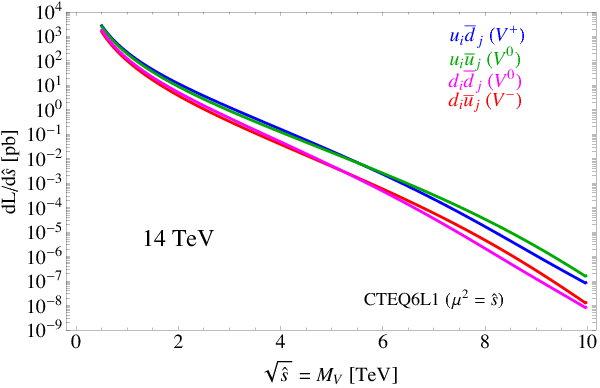
\includegraphics[width=.495\textwidth]{figures/Figures_LumiDY14.png}
  \caption{Parton luminosities for Drell-Yan process between $i$ and $j$ partons, as a function of the parton center-of-mass energy, for the LHC proton-proton collisions performed at 14 TeV.}
  \label{fig:HVT_DY_partolumi}
\end{figure}

\begin{figure}[!htb]
  \centering
    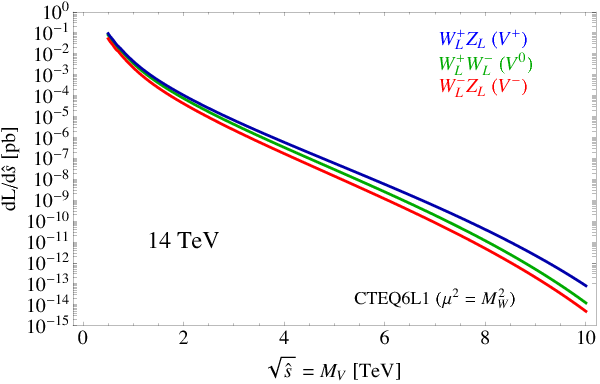
\includegraphics[width=.495\textwidth]{figures/Figures_LumiVBF14.png}
  \caption{Parton luminosities for VBF process between $i$ and $j$ partons, as a function of the parton center-of-mass energy, for the LHC proton-proton collisions performed at 14 TeV.}
  \label{fig:HVT_VBF_partolumi}
\end{figure}

\subsection{Benchmark model A: weak coupling scenario}
\label{sec:theory_HVT_A}
Model A scenario aims at reproducing a simple generalization of the SM~\cite{Barger:1980ix}, obtained by extending the gauge symmetry group with an additional $SU(2)'$. The low-energy phenonemna are expected to be dominated by the SM, while the high-energy processes are relevant for the additional symmetry, bringing additional light vector bosons in play.\\
It can be shown that this kind of picture is portrayed by HVT when $c_H \sim -g^2/g_V^2$ and $c_F \sim 1$. This implies that:
\begin{equation}
\begin{split}
 & g_V c_H \approx g^2/g_V\\
 & g^2 c_F/g_V \approx g^2/g_V,\\
\end{split}
\label{eq:theory_HVT_modelA}
\end{equation}
hence the partial decay in widths into fermions (eq.~\ref{eq:HVT_width_fermions}) and bosons (eq.~\ref{eq:HVT_width_dibosons}) differ only by a factor 2 and the colour factor ($N_c$). Branching fractions for the model A benchmark scenario ($g_V =1$) are shown in fig.~\ref{fig:HVT_modelA_BR_width} (left); total widths are reported in fig.\ref{fig:HVT_modelA_BR_width} (right) for different coupling parameters $g_V$.  

\begin{figure}[!htb]
  \centering
    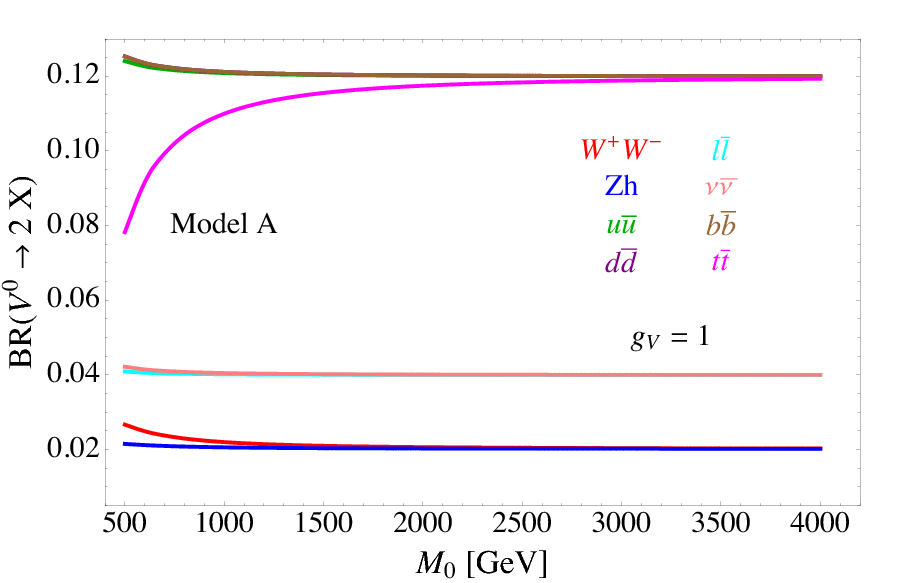
\includegraphics[width=.495\textwidth]{figures/Figures_BRWC.png}%
    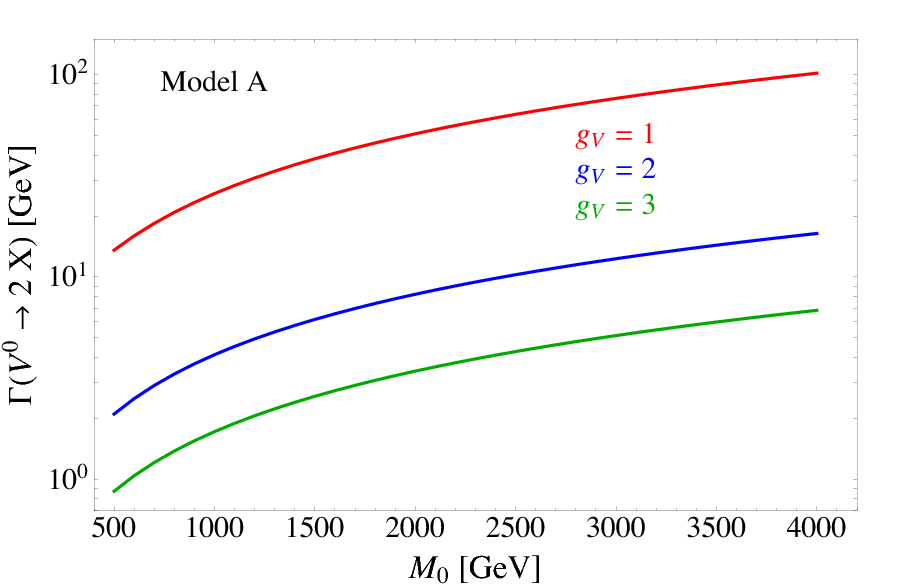
\includegraphics[width=.495\textwidth]{figures/Figures_WidthWC.png}
  \caption{HVT model A scenario: branching fractions for fermionic and bosonic decays when $g_V = 1$ (left) as a function of the mass of the resonance $M_0$; total width of the resonance, as a function of its mass, considering different values of the parameter $g_V$ (right).}
  \label{fig:HVT_modelA_BR_width}
\end{figure}

\subsection{Benchmark model B: strong coupling scenario}
\label{sec:theory_HVT_B}
In composite Higgs models~\cite{Contino2011}, the Higgs boson is the result of the spontaneous symmetry breaking of an $SO(5)$ symmetry to a $SO(4)$ group. New vector bosons are expected to appear, and the lightest ones can be represented by HVT model B when $c_H \sim c_F \sim 1$.\\ 
In this case:
\begin{equation}
\begin{split}
 & g_V c_H \approx -g_V\\
 & g^2 c_F/g_V \approx g^2/g_V,\\
\end{split}
\label{eq:theory_HVT_modelB}
\end{equation}
hence the decay into bosons is not suppressed by $g_V$ parameter. In the benchmark scenario $g_V=3$, decays into dibosons are largely dominant, as it can be seen in fig.~\ref{fig:HVT_modelB_BR_width} (left); the total decay width increases for larger $g_V$ (fig.~\ref{fig:HVT_modelB_BR_width}, right). When the resonances start to be very broad, \textit{i.e.} $\Gamma/M_V \gg 0.1$, the assumptions leading to the simplified model are no longer valid, hence higher order, non -resonant effects must be taken into account.

\begin{figure}[!htb]
  \centering
    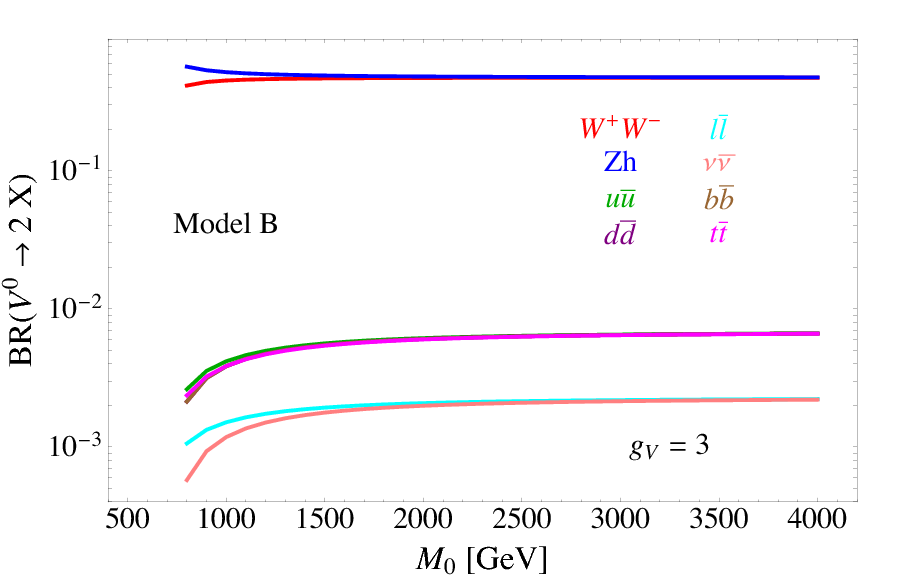
\includegraphics[width=.495\textwidth]{figures/Figures_BRSC.png}%
    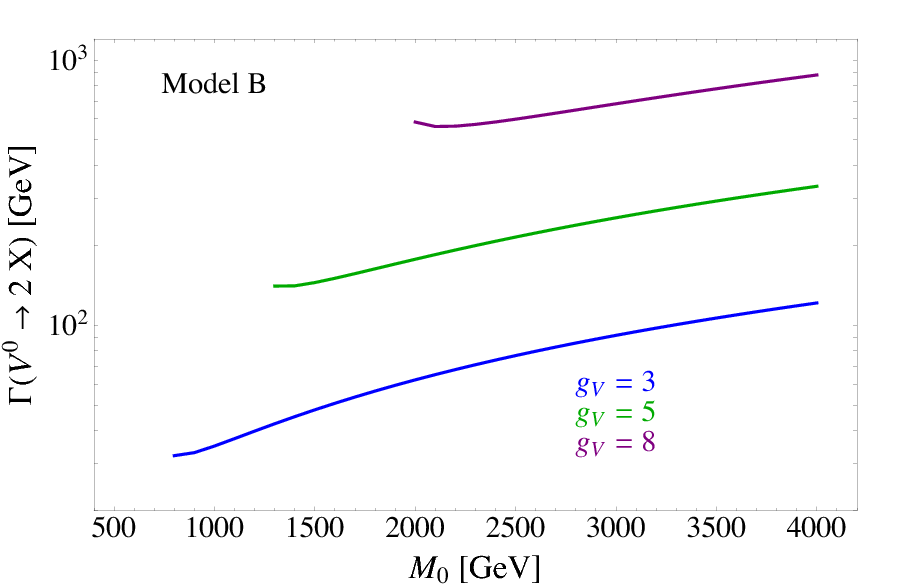
\includegraphics[width=.495\textwidth]{figures/Figures_WidthSC.png}
  \caption{HVT model B scenario: branching fractions for fermionic and bosonic decays when $g_V = 3$ (left) as a function of the mass of the resonance $M_0$; total width of the resonance, as a function of its mass, considering different values of the parameter $g_V$ (right).}
  \label{fig:HVT_modelB_BR_width}
\end{figure}

\subsection{HVT limits set by LHC at a center-of-mass energy of 8 TeV and perspectives at 14 TeV}
\label{sec:theory_HVT_limits_LHC_Run1}
Data collected by ATLAS and CMS experiments are used to set limits on the HVT resonance masses and coupling parameters. Experimental results, both from Run 1 LHC data (at a center-of-mass energy of 8 TeV) and Run 2 (at a center-of-mass energy of 13 TeV) will be discussed in detail in chapter~\ref{chap:LHC_CMS}.\\
A weakly coupled resonance, in the context of benchmark model A ($g_V = 1$) is excluded up to 3 TeV by Run 1 data. By looking at parton luminosities in fig.\ref{fig:HVT_DY_partolumi}, in data produced by LHC proton-proton collision at 14 TeV, collected for an integrated luminosity of 300 $\mbox{fb}^{-1}$, sensitivity should increase up to $m_V \approx 6$ TeV. A strongly coupled resonance, in the context of benchmark model B ($g_V = 3$) is excluded up to 2 TeV by Run 1 data. Data produced by LHC at 14 TeV should increase the sensitivity up to $m_V \approx 3-4$ TeV.
\newpage
\section{Warped extra dimension}
\label{sec:theory_WED}
The Randall-Sundrum model~\cite{Randall:1999ee,Randall:1999vf} (referred as RS1) proposes the introduction of one additional warped dimension in order to solve the hierarchy problem. The metric of the 5-dimensional space (a slice of $AdS_5$) generates an exponential hierarchy between the electroweak and Planck scales, associated to the TeV three-brane, where the SM particles are confined, and the Planck three-brane. As a consequence of the new geometry, spin-2 massive gravitons are predicted to exist.\\
The bulk extension of the Randall-Sundrum model~\cite{Agashe:2007zd,Fitzpatrick:2007qr} states that the SM fields can propagate in the extra dimension. Light fermions are near the Planck brane, heavy fermions are close to the TeV brane, while the Higgs sector is confined in the TeV brane. Higgs couplings to the heavy fermions are therefore expected to be stronger: this naturally arising hierarchy of the masses of the SM fields gives a solution to the flavour problem. In this scenario, the fermionic decays of the bulk gravitons are suppressed, while the bosonic decays are preferred.

\subsection{Randall-Sundrum original model (RS1)}
The existence of additional $n$-dimensions implies that the effective Planck scale observed in 4-dimensions, $M_{PL} = 1.2209 10^{19}$ GeV, is related to the fundamental (4+$n$) Planck scale, $M$, via the geometry. If the 4-dimensional and the $n$ additional metrics are factorizable, $M_{PL}$ is the product of $M$ and the volume of the compact space $V_n$:
\begin{equation}
M_{PL}^2 = V_n M^{2+n}.
\label{eq:theory_planck_mass}
\end{equation}
If $M \sim$ TeV, this implies than $V_n$ must be very large, hence the compactification scale $\mu \sim V_n^{1/n}$ is small (eV -- MeV for n=2 -- 7).  Given the smallness of the scale when compared to the electroweak scale, the effects of the extra dimension should be evident in SM processes. Since they are not observed, SM particles are assumed to be confined in a 4-dimensional space, the TeV three-brane, while only gravity is allowed to propagate into the 4+$n$-dimensional space, the bulk. This mechanism solves the hierarchy of the Higgs scale but introduces a new hierarchy between $\mu$ and $M$.\\
In the Randall-Sundrum model~\cite{Randall:1999ee,Randall:1999vf}, only one additional dimension is added. The geometry of the 5-dimensional bulk is non-factorizable, and it is a slice of $AdS_5$ spacetime.\footnote{An $n$-dimensional anti-de Sitter space ($AdS_n$) is a maximally simmetric Lorentiaz mainfold, that solves the Einstein equation with a negative curvature; it is a solution to the Einstein equation with negative cosmological constant.} The 4-dimensional metric is multiplied by an exponential function of the fifth dimension (the "warp" factor):
\begin{equation}
ds^2 = e^{-2 k r_c \phi} \eta_{\mu \nu} dx^{\mu} dx^{\nu} + r_c^2 d{\phi}^2;
\label{eq:theory_metric}
\end{equation}
$x^{\mu}$ are the usual 4-dimensional coordinates, $k$ is a scale (order of the Planck scale), $\phi$ is the coordinate of the extra dimension, $0 < |\phi| < \pi$, and $r_c$ is the compactification radius of this finite interval. 4-dimensional mass scales are obtained multiplying bulk masses by $e^{-2 k r_c \phi}$: given the exponential form of the warp factor, a small $r_c$ suffices for generating a large hierarchy between Planck and Higgs scales.

\subsection{Bulk extension of RS1}
\subsection{Bulk graviton production and decays}

\clearpage

